\documentclass{article}

%%% PREAMBLE %%%%%%%%%%%%%%%%%%%%%%%%%%%%%%%%%%%%%%%%%%%%%%%%%%%%%%%%%%%%%%%%%%%
% Load packages
\usepackage{fullpage} % Larger margins
\usepackage{cite} % Make references as [1-4], not [1,2,3,4]
\usepackage{amssymb,amsmath}
\usepackage{authblk}  % For author affiliations
\usepackage{hyperref}
\usepackage{graphicx}

% Macros
\newcommand{\hemaClass}{\href{http://hemaClass.org}{\texttt{hemaClass.org}}}

%%%%%%%%%%%%%%%%%%%%%%%%%%%%%%%%%%%%%%%%%%%%%%%%%%%%%%%%%%%%%%%%%%%%%%%%%%%%%%%%

\title{\hemaClass{}: an online based diffuse large B-cell lymphoma classification tool}

\author[1]{Steffen Falgreen}
\author[12]{Anders Ellern Bilgrau}
\author[1]{Tarec Christoffer El-Galaly}
\author[1]{Julie St{\o}ve  B{\o}dker}
\author[1]{Alexander Schmitz}
\author[1]{Malene Krag Kjeldsen}
\author[1]{Hans Erik Johnsen}
\author[1]{Karen Dybk{\ae}r}
\author[13]{Martin B{\o}gsted\thanks{To whom correspondence should be addressed (\texttt{sfl@rn.dk})}}

\affil[1]{Department of Haematology, Aalborg University Hospital}
\affil[2]{Department of Mathematical Sciences, Aalborg University}
\affil[3]{Department of Clinical Medicine, Aalborg University}

% Steffen Falgreen - sfl@rn.dk
% Anders Ellern Bilgrau - a.bilgrau@rn.dk
% Tarec Christoffer El-Galaly - tarec.galaly@gmail.com
% Julie S.\  B\o dker - j.boedker@rn.dk
% Alexander Schmitz - alex.schmitz@rn.dk
% Malene K.\ Kjeldsen - makrp@rn.dk
% Hans E.\ Johnsen - haej@rn.dk
% Karen Dybk\ae r - k.dybkaer@rn.dk
% Martin B\o gsted - martin.boegsted@rn.dk

\begin{document}

\maketitle
\phantomsection
\addcontentsline{toc}{section}{Abstract}
\begin{abstract}
\hemaClass{} Dozens of genomics based cancer classification systems have been introduced with prognostic, diagnostic, and predictive capabilities.
However, they are often based on complex algorithms only applicable on whole cohorts of patients, making them difficult to validate and apply.
This prompted us to create \hemaClass{} which is an online tool that provides an easy interface to one-by-one microarray based state-of-the-art risk classification of diffuse large B-cell lymphoma (DLBCL).
Focus has been put into pre-processing the array in a one-by-one manner compared to the usual normalisation in whole cohorts.
Such single sample normalisation is essential for establishing a clinically useful tool.
However, laboratory specific effects cannot be accounted for in one-by-one normalisation.
Hence, \hemaClass{} optionally allows the user to supply a reference dataset to increase the accuracy of the classifications.
Classification results for one-by-one array processing with and without a user supplied reference dataset were compared to cohort based classifiers in 4 publicly available datasets.
Overall, \hemaClass{} yields satisfactory inter-method agreements across all datasets.
\hemaClass{} is relevant for biological and clinical researchers in the lymphoma field as it provides a reliable and swift method for calculation of DLBCL subclasses.
\medskip\\
\textbf{Keywords:~}
Dose response experiments; NCI60; Doxorubicin; Mathematical modelling; Differential equation modelling; Nonlinear regression; Isotonic regression; Bootstrap; Parametric bootstrap
\end{abstract}



\section{Introduction}

%\subsection{Background}
In addition to current clinically used risk factor scoring systems several independent gene expression profile (GEP) based risk stratifications have been proposed with biological and clinical significance in DLBCL.
Although drug targetable genes which are only expressed in subtypes of the DLBCL tumours have been identified, they are not readily applicable in clinical research and routine settings due to lack of available routine diagnostic tests \cite{Jaffe2009}.

%\subsection{Motivation}
Alizadeh et al. \cite{Alizadeh2000} developed an important example of a biological sub-classification of lymphoma.
On the basis of gene expression profile analyses DLBCL cases were assigned to categories of activated B-cell phenotype (ABC) or germinal center B-cell phenotype (GCB) with different clinical outcomes.
The validity of this classification and its prognostic importance has been confirmed in a number of later studies \cite{Rosenwald2002a,Hans2004,Lenz2008a,Monti2012a}.
Recently, we have refined the ABC/GCB subclassification of DLBCL to include a B-cell Associated Gene Signature (BAGS) classifier capable of classifying DLBCL samples into 5 different B-cell subtypes: Naive (N), Centrocyte (CC), Centroblast (CB), Memory (M), and Plasmablasts (PB).
For example, the BAGS classifier stratifies the GCB subclass into a CC subtype with superior survival as compared to the CB subtype \cite{Dybkaer2013} which opens up for considering different treatment regimes in the GBC class of patients.
In another study \cite{Falgreen2013c} we developed classification based resistance gene signatures (REGS) for the most prominent drugs used in the treatment of DLBCL patients: Cyclophosphamide (C), Doxorubicin (H), and Vincristine (O).
However, these and most existing algorithms are only applicable in the presence of whole cohorts of patients making them difficult to apply in a clinical setting.

The traditional lymphoma staging and risk classification systems are based on the Ann Arbor classification for staging of lymphoma (extent of disease and extranodal involvement) and simple prognostic tools such as the IPI for large cell lymphoma and FLIPI for follicular lymphoma (both derived from patient age, performance status, easy available blood tests, and disease stage).
Risk stratification according to these algorithms have been systematised and made easily accessible for desktop, online, and even smart-phone use.
However, easily accessible molecular classification methods are lacking behind and thereby delaying the translation of new molecular findings into clinical practice.
A few methods exist for cancer types other than lymphoma, see e.g.\ \cite{Huang2009} for an AML application.
But to our knowledge, quite surprisingly, no tools have been developed for use in the lymphoma field despite very early promising results in the molecular biomarker field.
A single accessible Windows based application has recently been published for ABC/GCB classification \cite{Care2013}.
Although this method develops a new ABC/GCB classifier which is stable across a number of microarray technologies and trial centres it is biased for prognostic biomarkers.

This prompted us to develop an easy accessible and flexible web-based tool for ABC/GCB, BAGS, and REGS classification which is capable of computing our recently developed classifiers.
The classifications made by the web-based tool \hemaClass{} are compared to the existing state-of-the-art and approved ABC/GCB classifications of DLBCL.
We believe that \hemaClass{} will provide a novel and user-friendly concept for bringing complex molecular classification of disease swiftly into daily clinical practice.


\section{Materials and Methods}

\subsection{Classification workflow}
The analysis workflow of \hemaClass{} can be divided into four parts: (1) Three reference datasets which have been pre-processed and prepared offline are loaded upon server start, (2) a graphical user interface with upload and input facilities, (3) a server handling the online processing and classification of the user input, and (4) the resulting classifications available for download and inspection via the user interface.
This workflow architecture is illustrated in Figure \ref{fig:webtooldiagram}.

\begin{figure}
\begin{center}
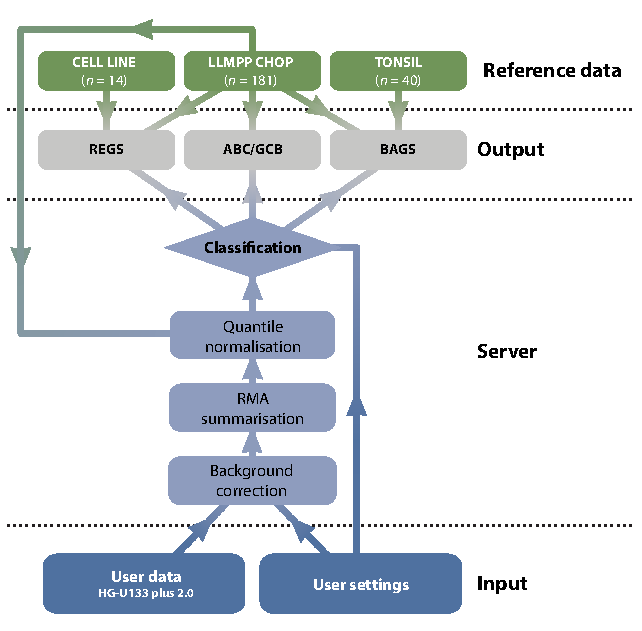
\includegraphics[width=0.5\textwidth]{Flowchart6.pdf}
\end{center}
\caption{Diagram of the workflow architecture.}
\label{fig:webtooldiagram}
\end{figure}

\subsection{Software}
The normalisation and classification procedures are implemented using the statistical programming language R \cite{RCoreTeam2013} and Bioconductor \cite{Gentleman2004}.
The interactive web application available at \url{http://hemaclass.org} was created using the R-package \texttt{shiny} \cite{RStudio2013} and the accompanying Linux server software.
The Shiny server handles the interaction between the front end web application and the back end R processing.

The RMA pre-processing was carried out with the Bioconductor package \texttt{affy} \cite{Gautier2004}.
%The code is open source and freely available for sharing, modification, and redistribution at GitHub (xxx).

\subsection{Data overview}
The seven gene expression datasets used in this article are summarised in Table \ref{table:01}.
All GEP data are on the Affymetrix GeneChip HG-U133 Plus 2.0 array and available at the Gene Expression Omnibus (GEO) website (www.ncbi.nlm.nih.gov/geo/query).
To establish the classifiers the following datasets are used:
\begin{enumerate}
  \item Gene expression data from 181 CHOP treated DLBCL patients are used to establish the ABC/GCB classifier.
  This cohort will be referred to as the Lymphoma/Leukemia Molecular Profiling Project CHOP cohort (LLMPP CHOP) \cite{Lenz2008a}.
  The cohort is also used as a reference set for normalisation of arrays.
  \item The BAGS classifier is based on gene expression data from eight human tonsils sorted in five B-cell subsets.
  This dataset will be referred to as the \textit{tonsil dataset} and it is also used for scaling of gene expression data for BAGS classification \cite{Dybkaer2013}.
  \item The REGS classifiers are based on a panel of 12 Multiple Myeloma (MM) and 14 DLBCL cell lines this panel will be referred to as BCELL26.
  The DLBCL part of the cell line panel is used for scaling of patient data and this part of the dataset will be referred to as \textit{DLBCL14} \cite{Falgreen2013c}.
\end{enumerate}
For validation the following DLBCL cohorts are used:
\begin{enumerate}
  \item[4] The Aalborg OCT (CHEPRETRO) cohort of 89 Danish DLBCL patients undergoing first-line treatment at the university  hospital of Aalborg.cite{Dybkaer2013}.
  The clinical dataset is as registered in the National Clinical Quality Database for Malignant Lymphoma (LYFO www.lymphoma.dk) \cite{Gang2012}.
  \item[5] The International DLBCL Rituximab-CHOP Consortium MD Anderson (IDRC) cohort of 470 DLBCL patients treated with R-CHOP first-line therapy.
  Detailed information about the cohort can be found in \cite{Visco2012}.
  \item[6] The Lymphoma/Leukemia Molecular Profiling Project R-CHOP (LLMPP R-CHOP) cohort of 233 DLBCL patients treated with R-CHOP first-line therapy.
  Details about the dataset can be found in \cite{Lenz2008a}.
  \item[7] The Mayo-Dana-Farber Cancer Institute (MDFCI) cohort of 90 DLBCL patients treated with R-CHOP first-line therapy \cite{Monti2012a}.
\end{enumerate}


\begin{table}%[htb]
\small
\caption{Overview of the GEO accession numbers for the used datasets.}
\label{table:01}%
\begin{center}
\begin{tabular}{lllll}
\hline\hline
Dataset & $n$ & Usage & GEO number & Ref.
\\
\hline
LLMPP CHOP & 181 & Reference & GSE10846 & \cite{Lenz2008a}
\\
Tonsil & 33 & Reference & - & \cite{Dybkaer2013}
\\
DLBCL14 & 14 & Reference & - & \cite{Falgreen2013c}
\\
CHEPRETRO & 89 & Validation & - & \cite{Dybkaer2013}
\\
IDRC & 470 & Validation & GSE31312 & \cite{Visco2012}
\\
LLMPP R-CHOP & 233 & Validation & GSE10846 & \cite{Lenz2008a}
\\
MDFCI & 90 & Validation & GSE34171 & \cite{Monti2012a}\\
\hline
\end{tabular}
\end{center}
\end{table}

\subsection{One-by-one RMA normalization}
Recall that RMA pre-processing consists of three steps: 1) Background correction, 2) quantile normalisation, and 3) summarisation of probes to probe-sets \cite{Irizarry2003}.
Both the normalisation and summarisation procedures of RMA are cohort based and hence need to be altered to facilitate a one-by-one RMA pre-processing scheme.
As quantile normaliser the empirical cumulative distribution function (ECDF) of the RMA background corrected LLMPP CHOP reference data is used in place of the usually applied ECDF of the mean of the sample quantiles \cite{Bolstad2003}.
To mimic the summarisation procedure of RMA \cite{Irizarry2003b} the probe effects estimated by median polish for the LLMPP CHOP reference data is subtracted all probes of the user data.
The RMA pre-processed expression value for each probe-set is then estimated as the median of the associated probes.

Finally, the median of each probe-set in the LLMPP CHOP is subtracted from the corresponding probe-set in the user data.
This ensures identical classification probabilities whether data is supplied as a cohort or one-by-one.

To accommodate laboratory and sample preparation specific effects different from the LLMPP CHOP reference data, \hemaClass{} allows the user to upload an alternative dataset which is to be used in place of LLMPP CHOP as reference.
In this article the reference datasets have consisted of 30 samples.

The three pre-processing methods will be referred to as cohort, one-by-one, and reference based normalisation.

\subsection{Classification methods}

\subsubsection{Elastic nets}
Logistic and multinomial regression are used in all classification methods available on \hemaClass{}.
However, in GEP experiments, the number of probe-sets present on the microarray always outnumbers the sample size.
Collinearity present among the features further aggravates the problem of identifying genes responsible for the underlying biological mechanism.
Regression under these ill-posed circumstances is typically handled by so-called regularisation.
Here the elastic net penalty \cite{Friedman2010, Zou2005} is used which is a combination of the lasso \cite{Tibshirani1996} and ridge regression \cite{Hoerl1970}.
Similar to the lasso this penalty ensures simultaneous variable selection and model estimation.
In contrast to the lasso the elastic net penalty is capable of selecting more variables than samples.
Regression with elastic net ensures sparse solutions by forcing small coefficients to be zero.

The elastic net penalty contains two parameters $\alpha$ and $\lambda$.
The parameter $\alpha$ interpolates the elastic net penalty between the ridge and the lasso penalty which corresponds to values of 0 and 1, respectively.
The parameter $\lambda$ determines the amount of shrinkage of the coefficients with larger values inducing more shrinkage until no variables are contained in the model.
Regularised logistic and multinomial regression are performed with the R-package \texttt{glmnet} \cite{Friedman2010}.

\subsubsection{ABC/GCB classification}
The ABC/GCB classifier is established using logistic regression with an elastic net penalty on the LLMPP CHOP cohort.
Of the 181 patients 74 were ABC, 76 were GCB and 31 were non-classified.
Using the 150 patients classified as either ABC or GCB the dichotomous classifier capable of assigning each sample an estimate of the probability of being ABC was established.

To avoid over-fitting and limit the number of noise contributing genes, the elastic net parameters $\alpha$ and $\lambda$ were chosen through 10 fold cross-validation.
The parameter $\alpha$ was varied between 0.1 and 1 with step size $0.025$ and $\lambda$ was varied between -10 and 2 with step size $0.06$.
The optimal combination of the parameters and thereby the number of probe-sets were found at the values minimising the deviance.
The results of the cross validation are shown in Supplementary Figure \ref{fig:crossval}.
The minimum 0.13 was attained at $\alpha$ equal to 0.15 and log($\lambda$) equal to -7.41 resulting in a gene expression classifier consisting of 381 probe-sets.

When a tumour sample is classified according to the ABC/GCB classifier using reference based normalisation the associated gene expressions are probe-set wise rescaled by the standard deviation of the LLMPP CHOP data divided by the standard deviation of the user supplied reference data.
In contrast, the one-by-one normalised data is used directly.

\subsubsection{REGS classification}
In the paper by Falgreen et al. \cite{Falgreen2013c} REGS classifiers were established for prediction of resistance to the drugs C, H, and O.
The classifiers were established on BCELL26 using regularised logistic regression analogous to the procedure described for the abovementioned ABC/GCB classifier.

The probability of resistance to the combination therapy CHO is estimated based on the probabilities of drug resistance toward the three drugs C, H, and O.
This probability is calculated by a formula derived as the posterior probability of being resistant given resistance towards each of the individual drugs under the assumption of drug independence.
The formula is also known as Graham's formula: $\mbox{CHO}/(\mbox{CHO}+(1-\mbox{C})(1-\mbox{H})(1-\mbox{O}))$.
If a drug is left out in the combination therapy the drug is simply removed from the formula.

When a tumour sample is classified according to the REGS classifiers the associated gene expressions are probe-set wise rescaled by the standard deviation of DLBCL14 divided by the standard deviation of the LLMPP CHOP dataset.
Similarly to the other classifiers the LLMPP CHOP cohort is replaced by the user reference dataset, if supplied.


\subsubsection{BAGS classification}
The BAGS classifier established by Dybk{\ae}r et al. \cite{Dybkaer2013} was based on multinomial regression regularised by an elastic net penalty.
The classifier was trained on the Tonsil dataset in a manner similar to the ABC/GCB classifier.

When a tumour sample is classified according to the BAGS classifier the associated gene expressions are probe-set wise rescaled by the standard deviation of the tonsil data divided by the standard deviation of the LLMPP CHOP dataset.
If the user supplies a reference dataset this is used in place of LLMPP CHOP.
The rescaling is performed to make the data comparable to the tonsil dataset.


\subsection{Inter method reproducibility assessments}
To evaluate the reproducibility of the class probabilities obtained through cohort based normalisation and hemaclas.com normalisation Pearson's correlation coefficient for the logit-transformed probabilities and 95\% confidence interval (CI) were calculated for each classifier and dataset.
The identity and orthogonal least square regression lines were compared to assess bias in estimated probabilities \cite{CHEN1989}.
Orthogonal regression was used because errors in both classification probabilities are present.

For each classifier the associated categories were obtained by thresholding the estimated probabilities.
The ABC/GCB classifier was thresholded by 0.1 and 0.9, i.e.\ a tumour sample was classified as ABC when the estimated probability exceeds 0.9, GCB when it is beneath 0.1, and unclassified otherwise.
For the BAGS classifier a tumour was classified as N, CB, CC, M, or PB if the associated probability exceeded 0.5 and unclassified when this threshold was not met for any subtype.
For the REGS classifier, C, H, O, and CHO combined the 33\% and 66\% percentile of the estimated probabilities were $[0.46, 0.67]$, $[0.1, 0.86]$, $[0.38, 0.54]$, and $[0.07, 0.91]$.
After thresholding the class probabilities confusion matrices were created.
From these accuracy or rate of agrement, Cohen's $\kappa$, and corresponding 95\% CIs were computed to assess the agreement between the determined classes.


\section{Results}
\subsection{Usage of \hemaClass{}}
\hemaClass{} has an easy-to-use interface with a single data query field and the possibility to select between classification methods.
The classifications made by \hemaClass{} using the one-by-one and reference based normalisations are compared to that obtained by means of cohort based normalisation in the following sections.

\subsection{ABC/GCB classification}
In order to classify patients as ABC/GCB based on the implemented one-by-one normalisation method a classifier based on regularised logistic regression was established.

The classifications made by this classifier were evaluated in the four clinical cohorts CHEPRETRO, MDFCI, IDRC, and LLMPP R-CHOP, which have all been classified according to Wright's method \cite{Wright2003,Lenz2008a}.
The rate of agreement between the two classifiers are shown in Table \ref{tab:ABCGCBclassifier}.
Note that unclassified samples were included in the estimation of this rate i.e.\ a patient classified as ABC by one classifier but unclassified by the other is considered an error.
The table also includes weighted Cohen's $\kappa$ estimates.
Here misclassifications involving the unclassified group are weighted by 0.5.
The accompanying confusion matrices are shown in Supplementary Table \ref{tab:confusionABCGCBHEMA}.

The logit probability of being ABC estimated using the established classifier was compared to the estimate obtained through the one-by-one classification scheme in Figure \ref{fig:ABCGCBDrug}A for CHEPRETRO.
The rank of the probabilities estimated through the two methods are very similar, however, the probabilities estimated through \hemaClass{} are skewed upwards, indicating that different cut points should be used for classification.
By normalising to a reference set of 30 randomly selected samples from CHEPRETRO this error is greatly minimised as shown in Figure \ref{fig:ABCGCBDrug}B.

For both methods patients are classified as ABC when the estimated probability exceeds 0.9 and GCB when it is below 0.1.
In Table \ref{tab:classALL} the resulting classifications are compared in terms of accuracy and weighted Cohen's $\kappa$ for the four cohorts: CHEPRETRO, MDFCI, IDRC, and LLMPP R-CHOP showing good agreement, even considering that misclassifications involving unclassified samples count as errors, albeit weighted by 0.5 in Cohen's $\kappa$.
The accompanying confusion matrices are shown in Supplementary Table \ref{tab:confusionABCGCBHEMA}.

\begin{table}
\small
\caption{Comparison of ABC/GCB classification performed using Wright's method and the established classifier based on cohort normalisation for both.
The first column shows the rate of agreement between the classifiers with 95\% CI.
The second column shows the Cohen's $\kappa$ with 95\% CI.\label{tab:ABCGCBclassifier}}
\begin{center}
\begin{tabular}{lll}
\hline\hline
\multicolumn{1}{l}{Cohort}&\multicolumn{1}{c}{Rate of agrement}&\multicolumn{1}{c}{Cohen's $\kappa$}\tabularnewline
\hline
CHEPRETRO&0.93 (0.86,0.97)&0.84 (0.76,0.92)\tabularnewline
MDFCI&0.89 (0.81,0.95)&0.81 (0.69,0.94)\tabularnewline
IDRC&0.82 (0.78,0.85)&0.67 (0.63,0.71)\tabularnewline
LLMPP R-CHOP&0.9 (0.86,0.94)&0.8 (0.74,0.86)\tabularnewline
\hline
\end{tabular}
\end{center}
\end{table}



%

\begin{figure}
\begin{center}
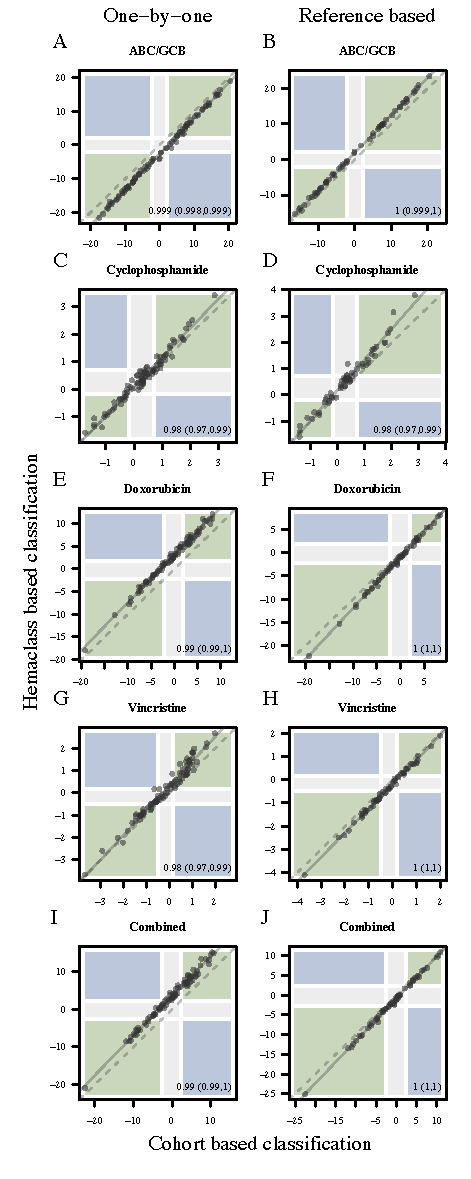
\includegraphics[width=0.375\textwidth]{DruglogitChep.pdf}
\end{center}
\caption{Comparison of logit probabilities for ABC/GCB and REGS classification obtained through cohort normalisation and \hemaClass{}.
The areas marked with green indicate patients with similar classification between \hemaClass{} and cohort based normalisation.
Contrary, the areas marked with blue indicate misclassification.
For ABC/GCB and REGS the grey areas indicate unclassified and intermediate resistant, respectively.}
\label{fig:ABCGCBDrug}
\end{figure}

\begin{figure}
\begin{center}
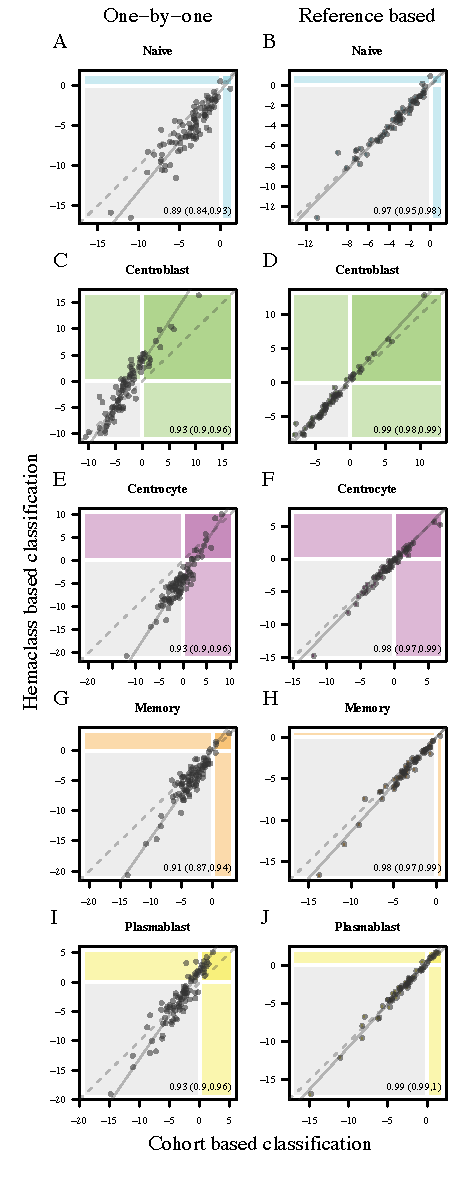
\includegraphics[width=0.375\textwidth]{BAGSlogitChep.pdf}
\end{center}
\caption{Comparison of logit probabilities for the BAGS classifier obtained through cohort normalisation and \hemaClass{}.
The coloured regions in the figure correspond to a threshold probability of 0.5.}
\label{fig:Bagscorr}
\end{figure}
\newpage


\subsection{REGS classification}

The probability of resistance toward the three drugs C, H, and O was estimated using \hemaClass{} both in terms of one-by-one and reference based normalisation.
The logit probabilities are plotted against those obtained by cohort based normalisation in Figure \ref{fig:ABCGCBDrug}.
Panels C, E, G, and I show the plots based on one-by-one normalisation and panels D, F, H, and J show the plots for the reference based normalisation.
The probabilities obtained by one-by-one and cohort based normalisation are comparable, however, similar to the other classifiers the one-by-one normalisation leads to skewed probabilities, indicating that different cut points should be used.

The probabilities obtained by the reference based normalisation resembles the cohort based to a great extent indicating that similar probabilities are obtainable for different laboratories by supplying a reference set.

Based on the estimated probabilities the patients were categorised as sensitive, intermediate, or resistant based on the thresholds specified in the methods section.
The classes obtained by \hemaClass{} are compared to those obtained by the cohort based approach in Table \ref{tab:classALL} in terms of accuracy and Cohen's $\kappa$.
The associated confusion matrices for one-by-one normalisation and reference based normalisation are shown in Supplementary Table \ref{tab:confusiondrugonebyone} and Supplementary Table \ref{tab:confusiondrugreference}, respectively.

\subsection{BAGS classification}

The BAGS classifier was evaluated in a manner similar to the ABC/GCB classifier.
The logit probability of a patient's tumour originating from one of the five subpopulations is estimated by means of cohort, one-by-one, and reference based normalisation.
The logit probabilities estimated by the one-by-one normalisation is plotted against that estimated for the cohort based normalisation in Figure \ref{fig:Bagscorr} panels A, C, E, G, and I for CHEPRETRO.
The correlation between the logit probabilities is highly significant, although skewed.
To accommodate this, the data was also normalised using a reference dataset.
The logit probabilities estimated by the reference based normalisation is plotted against that estimated for the cohort based normalisation in Figure \ref{fig:Bagscorr} panels B, D, F, H, and J for CHEPRETRO.
The reference based normalisation removes much of the aforementioned bias.

Based on the probabilities estimated by means of each of the three normalisation methods the patients of the four clinical cohorts are grouped into the BAGS.
The rate of agreement between the cohort based and \hemaClass{} classifications is shown in Table \ref{tab:classALL} along with the weighted Cohen's $\kappa$.
The associated confusion matrices are shown in Supplementary Table \ref{tab:BAGShemaclass}.



\begin{table}[!tbp]
\scriptsize
\tabcolsep=0.11cm
\caption{Comparison of classifications obtained using cohort based normalisation and \hemaClass{}.
The classifications are compared in terms of accuracy, Cohen's $\kappa$, and Pearson's correlation coefficient $\rho$ all supplied with 95\% CIs.
The comparisons in the first and last three columns are based on the one-by-one normalisation method and the reference based normalisation method, respectively.\label{tab:classALL}}
\begin{center}
\begin{tabular}{llllclll}
\hline\hline
\multicolumn{1}{l}{\bfseries }&\multicolumn{3}{c}{\bfseries One-by-one normalisation}&\multicolumn{1}{c}{\bfseries }&\multicolumn{3}{c}{\bfseries Reference based normalisation}\tabularnewline
\cline{2-4} \cline{6-8}
\multicolumn{1}{l}{}&\multicolumn{1}{c}{Accuracy}&\multicolumn{1}{c}{Cohens's $\kappa$}&\multicolumn{1}{c}{Pearson's $\rho$}&\multicolumn{1}{c}{}&\multicolumn{1}{c}{Accuracy}&\multicolumn{1}{c}{Cohen's $\kappa$}&\multicolumn{1}{c}{Pearson's $\rho$}\tabularnewline
\hline
{\bfseries ABC/GCB}&&&&&&&\tabularnewline
~~CHEPRETRO&0.87 (0.78,0.93)&0.71 (0.64,0.77)&0.999 (0.998,0.999)&&0.92 (0.81,0.97)&0.82 (0.72,0.92)&1 (0.999,1)\tabularnewline
~~MDFCI&0.68 (0.57,0.77)&0.47 (0.37,0.57)&0.998 (0.998,0.999)&&0.9 (0.79,0.96)&0.86 (0.7,1)&0.974 (0.957,0.984)\tabularnewline
~~IDRC&0.64 (0.59,0.68)&0.27 (0.22,0.31)&0.985 (0.982,0.987)&&0.76 (0.72,0.8)&0.59 (0.55,0.64)&0.987 (0.984,0.989)\tabularnewline
~~LLMPP R-CHOP&0.83 (0.77,0.87)&0.62 (0.58,0.67)&0.999 (0.999,0.999)&&0.94 (0.9,0.97)&0.88 (0.81,0.95)&1 (0.999,1)\tabularnewline
\hline
{\bfseries BAGS}&&&&&&&\tabularnewline
~~CHEPRETRO&0.55 (0.44,0.66)&0.5 (0.24,0.77)&-&&0.9 (0.79,0.96)&0.88 (0.54,1)&-\tabularnewline
~~MDFCI&0.5 (0.39,0.61)&0.45 (0.14,0.76)&-&&0.82 (0.7,0.9)&0.81 (0.33,1)&-\tabularnewline
~~IDRC&0.48 (0.43,0.52)&0.39 (0.3,0.48)&-&&0.77 (0.73,0.81)&0.77 (0.64,0.89)&-\tabularnewline
~~LLMPP R-CHOP&0.57 (0.5,0.64)&0.54 (0.37,0.71)&-&&0.69 (0.62,0.75)&0.67 (0.46,0.87)&-\tabularnewline
\hline
{\bfseries REGS}&&&&&&&\tabularnewline
~~CHEPRETRO&0.62 (0.51,0.72)&0.58 (0.46,0.71)&0.99 (0.99,1)&&0.93 (0.84,0.98)&0.92 (0.77,1)&1 (1,1)\tabularnewline
~~MDFCI&0.43 (0.33,0.54)&0.35 (0.23,0.46)&0.99 (0.99,0.99)&&0.78 (0.66,0.88)&0.76 (0.61,0.91)&1 (1,1)\tabularnewline
~~IDRC&0.64 (0.6,0.68)&0.57 (0.52,0.62)&0.94 (0.93,0.95)&&0.91 (0.88,0.93)&0.89 (0.84,0.95)&0.98 (0.98,0.99)\tabularnewline
~~LLMPP R-CHOP&0.42 (0.36,0.49)&0.32 (0.25,0.38)&0.99 (0.98,0.99)&&0.87 (0.81,0.91)&0.85 (0.77,0.93)&1 (1,1)\tabularnewline
\hline
\end{tabular}
\end{center}
\end{table}


\section{Discussion}
Despite the enormous resources spent on developing molecular based cancer classification systems there seems to be an inertial resistance to develop clinical applications.
To allow for fast validation of our recent findings \cite{Dybkaer2013, Falgreen2013c}, we have developed an easily accessible web application that permits other users to apply ABC/GCB, BAGS as well as drug resistance classification on their own datasets.

The classifications performed by \hemaClass{} were compared to those obtained using cohort based normalisation in four clinical cohorts.
Even though gene expression data for the four cohorts was obtained through varying preparation kits and sample storage methods, the results show that a one-by-one array analysis approach performed comparably with the whole cohort based method.
It seems that this approach allows for a realistic application of microarray based lymphoma classification for research projects and, after suitable standardisation, even for clinical use.

The present treatment algorithms for DLBCL are based on disease stage and clinical risk stratification without account of underlying tumour-biology \cite{Schmoll2012}.
The CHOP combination therapy (cyclophosphamide, doxorubicin, vincristine, and prednisone) has been the backbone of DLBCL therapy for decades with the only significant improvement being the addition of monoclonal CD20 antibodies (rituximab) \cite{Coiffier2002a}.
Despite the addition of antibody therapy to conventional chemotherapy only 55\% of patients with poor risk disease achieve durable remission \cite{Ziepert2010}.
Thus, the need for new therapeutic options in DLBCL is obvious.
Currently a number of new drugs have shown promising activity in DLBCL, but their role outside clinical trials has not been defined.
These drugs are different from conventional chemotherapeutic compounds by targeting specific deregulated cell-cycle pathways \cite{Friedberg2011}.
An important example is inhibition of the NF-$\kappa\beta$ pathway by proteasome inhibitors (i.e.\ bortezomib).
Interestingly, the constitutive activation of the NF-$\kappa\beta$ pathway is characteristic for the ABC subtype of DLBCL and consistently bortezomib more activity in this subtype \cite{Nogai2013}.
With the increasing number of new drugs likely to become available over the next years and the fact that their efficacy may vary between subsets of patients defined by gene expression profiles, the current treatment of patients based on disease stage and clinical information alone will not be sufficient.
\hemaClass{} provides an example of fast processing of complex molecular information in a way that is simple and readily at hand for clinicians.

An immediate limitation of the study is the need for a reference data set run under the same conditions as the samples one wishes to classify.
However, calibration of laboratory equipment is a well-known issue for many experimental techniques used in molecular biology like qPCR, mass spectrometry, immunohistochemistry, and flow cytometry.
An important part of the calibration is that samples should be calibrated towards a dataset consisting of a representative set of tissue samples.
For the microarray technology this could be solved by inventing a central tissue bank of e.g.\ B-cell cancer cell-lines of varying subtypes which could be used as reference set for each individual microarray platform.

The user reference data set is important if one wish to use the conventionally used thresholds for classification.
However without a user reference set, the high correlation coefficients demonstrate that equally high classification accuracies can be achieved if laboratory specific thresholds are carefully chosen.

Another limitation of the current web application is that it is only designed for one array type.
This can, however, be circumvented by either re-annotation to HUGO Gene Nomenclature Committee (HGNC) approved symbols as suggested by Care et al. \cite{Care2013} or by re-annotated chip definition files as suggested by \cite{Dai2005}.
At the moment we are working on extending the web application to other array types along these lines.

Traditionally ABC/GCB classification has been achieved using Wright et al.'s method \cite{Wright2003} which is based on cohorts, MAS5.0 normalised arrays, and a Bayesian approach assuming an equal amount of ABC and GCB patients.
However, a classifier based on logistic regression regularised by an elastic net penalty was implemented to make the classification more adaptable to RMA normalisation, one-by-one processing, and stable towards varying amounts of ABC/GCB patients.
This classifier proved to be quite comparable with Wright's classifier over the four studied datasets confirming the strong and stable signal of the ABC/GBC subclasses of DLBCL.

Under the validation of the one-by-one method one should notice that the unclassified is treated as a class in its own right.
This implies a lower accuracy compared to an approach where the unclassified are left out of the validations.
The latter approach seems reasonable as changing classifications to unclassified is less serious than changing real classes.
Despite the disputed properties of Cohen's $\kappa$ the conservative approach is retained and the issue is addressed using a weighted Cohen's $\kappa$ approach.
Given that an idealised approach is problematic to formulate, readers are encouraged to consider the confusion matrices in the supplementary material to make an overall evaluation of the performance.

ABC/GCB, BAGS, and REGS are only a part of the GEP-based armamentarium of methods for stratifying lymphoma patients into risk groups and it would be interesting to extend the tool to include other classification systems like e.g.\ \cite{Shipp2002, Lossos2004a, Malumbres2008} and for a comprehensive review see \cite{Coutinho2013}.
To our knowledge only a few other classification methods from other cancer types have been made easily accessible as either web applications or desktop applications.
Hopefully this research will inspire bioinformaticians and statisticians to make their cancer classification methods easily accessible for usage, speedy validation, critical reviews, and mutual inspiration.

\section{Conclusion}
Despite high throughput molecular biology has been around for more than a decade, only a few of the numerous biomarkers identified have undergone extensive validation and made it into the clinic \cite{Chen2012a}.
It is our hope that making our own findings publicly available in this way will speed up validation and testing of BAGS and REGS by other researchers without having to delve into extensive bioinformatics implementations.
Although \hemaClass{} is still separated from the clinic we believe a web based tool and suggestion for a clinical reference sample will bring cancer classification closer to the clinic.
Hopefully, this work can also spawn interesting discussions on the clinical requirements of GEP based diagnostic and prognostic tools.

\phantomsection
\addcontentsline{toc}{section}{Acknowledgements}
\section*{Acknowledgements}
SF is supported by a Mobility PhD fellowship at the Graduate School of Health, Faculty of Health Sciences, Aarhus University.
The research is supported by MSCNET, a translational programme studying cancer stem cells in multiple myeloma supported by the EU FP6, and CHEPRE, a programme studying chemo sensitivity in malignant lymphoma by genomic signatures supported by the Danish Agency for Science, Technology, and Innovation as well as Karen Elise Jensen Fonden.
The technical assistance from Ann-Maria Jensen, Louise Hvilsh{\o}j Madsen, and Helle H{\o}holt is greatly appreciated.


\noindent\textit{Conflict of interest statement}: None declared.
\phantomsection
\addcontentsline{toc}{section}{References}
\bibliographystyle{plain}
\bibliography{library2}



\begin{figure*}[htb]
\begin{center}
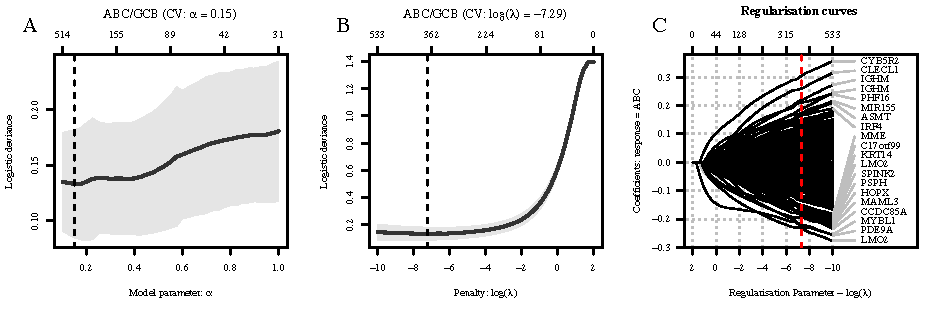
\includegraphics[width=1\textwidth]{CrosvalidationClass.pdf}
\end{center}
\caption{Ten fold cross validation for the parameters $\alpha$ and $\lambda$ for logistic regression regularised by elastic net.
In panels A and B the deviance is plotted against the model parameter $\alpha$ and regularisation parameter $\lambda$, respectively.
In Panel C the regularisation curves are shown.
Black and grey curves represent selected and nonselected probe-sets.
Positive and negative coefficients indicate that high expression values for the associated gene are related to ABC and GCB, respectively.
The red line indicates the model chosen through 10 fold cross validation.
The gene symbols for the 20 probe-sets associated with the largest absolute coefficients in the chosen gene expression predictors are displayed.}
\label{fig:crossval}
\end{figure*}

\begin{table*}[!tbp]
\footnotesize
\caption{Confusion tables for the ABC/GCB classifiers.
The columns represent cohort based normalisation using the ABC/GCB classifier based on elastic net.
The first part of the table compares Wright's method for ABC/GCB classification with the elastic net based.
In the second and third part one-by-one and reference based normalisation is compared to cohort based normalisation using the ABC/GCB classifier based on elastic net.\label{tab:confusionABCGCBHEMA}}
\begin{center}
\begin{tabular}{lrrrcrrrcrrrcrrr}
\hline\hline
\multicolumn{1}{l}{\bfseries  }&\multicolumn{3}{c}{\bfseries MDFCI}&\multicolumn{1}{c}{\bfseries }&\multicolumn{3}{c}{\bfseries IDRC}&\multicolumn{1}{c}{\bfseries }&\multicolumn{3}{c}{\bfseries LLMPP RCHOP}&\multicolumn{1}{c}{\bfseries }&\multicolumn{3}{c}{\bfseries CHEPRETRO}\tabularnewline
\cline{2-4} \cline{6-8} \cline{10-12} \cline{14-16}
\multicolumn{1}{l}{}&\multicolumn{1}{c}{ABC}&\multicolumn{1}{c}{NC}&\multicolumn{1}{c}{GCB}&\multicolumn{1}{c}{}&\multicolumn{1}{c}{ABC}&\multicolumn{1}{c}{NC}&\multicolumn{1}{c}{GCB}&\multicolumn{1}{c}{}&\multicolumn{1}{c}{ABC}&\multicolumn{1}{c}{NC}&\multicolumn{1}{c}{GCB}&\multicolumn{1}{c}{}&\multicolumn{1}{c}{ABC}&\multicolumn{1}{c}{NC}&\multicolumn{1}{c}{GCB}\tabularnewline
\hline
{\bfseries Wright's method}&&&&&&&&&&&&&&&\tabularnewline
~~ABC&$28$&$ 2$&$ 0$&&$176$&$23$&$  0$&&$89$&$ 4$&$  0$&&$38$&$2$&$ 0$\tabularnewline
~~NC&$ 2$&$19$&$ 1$&&$  6$&$26$&$ 12$&&$ 6$&$19$&$  8$&&$ 1$&$4$&$ 0$\tabularnewline
~~GCB&$ 0$&$ 5$&$33$&&$  6$&$38$&$183$&&$ 0$&$ 5$&$102$&&$ 0$&$3$&$41$\tabularnewline
\hline
{\bfseries One-by-one}&&&&&&&&&&&&&&&\tabularnewline
~~ABC&$23$&$ 0$&$ 0$&&$ 89$&$ 0$&$  0$&&$76$&$ 0$&$  0$&&$34$&$0$&$ 0$\tabularnewline
~~NC&$ 7$&$ 4$&$ 0$&&$ 95$&$15$&$  0$&&$19$&$ 7$&$  0$&&$ 5$&$2$&$ 0$\tabularnewline
~~GCB&$ 0$&$22$&$34$&&$  4$&$72$&$195$&&$ 0$&$21$&$110$&&$ 0$&$7$&$41$\tabularnewline
\hline
{\bfseries Reference based}&&&&&&&&&&&&&&&\tabularnewline
~~ABC&$17$&$ 0$&$ 0$&&$177$&$43$&$  0$&&$85$&$ 6$&$  0$&&$26$&$2$&$ 0$\tabularnewline
~~NC&$ 1$&$13$&$ 0$&&$  1$&$38$&$ 58$&&$ 0$&$20$&$  6$&&$ 0$&$3$&$ 3$\tabularnewline
~~GCB&$ 0$&$ 5$&$24$&&$  0$&$ 2$&$121$&&$ 0$&$ 0$&$ 86$&&$ 0$&$0$&$25$\tabularnewline
\hline
\end{tabular}
\end{center}
\end{table*}


\begin{table*}[!tbp]
\small
\caption{\textbf{Confusion tables for the BAGS classifier.} One-by-one and reference based normalisation are shown in the columns and cohort normalisation in the rows.\label{tab:BAGShemaclass}}
\begin{center}
\begin{tabular}{lrrrrrrcrrrrrr}
\hline\hline
\multicolumn{1}{l}{\bfseries  }&\multicolumn{6}{c}{\bfseries One-by-one normalisation}&\multicolumn{1}{c}{\bfseries }&\multicolumn{6}{c}{\bfseries Reference based normalisation}\tabularnewline
\cline{2-7} \cline{9-14}
\multicolumn{1}{l}{}&\multicolumn{1}{c}{N}&\multicolumn{1}{c}{CB}&\multicolumn{1}{c}{CC}&\multicolumn{1}{c}{M}&\multicolumn{1}{c}{PB}&\multicolumn{1}{c}{NC}&\multicolumn{1}{c}{}&\multicolumn{1}{c}{N}&\multicolumn{1}{c}{CB}&\multicolumn{1}{c}{CC}&\multicolumn{1}{c}{M}&\multicolumn{1}{c}{PB}&\multicolumn{1}{c}{NC}\tabularnewline
\hline
{\bfseries MDFCI}&&&&&&&&&&&&&\tabularnewline
~~Naive&$1$&$ 0$&$  0$&$1$&$ 5$&$0$&&$6$&$ 1$&$  0$&$ 0$&$ 0$&$ 0$\tabularnewline
~~Centroblast&$0$&$16$&$  0$&$0$&$ 0$&$0$&&$1$&$12$&$  0$&$ 0$&$ 0$&$ 0$\tabularnewline
~~Centrocyte&$0$&$ 6$&$  9$&$2$&$11$&$3$&&$0$&$ 1$&$ 15$&$ 0$&$ 1$&$ 1$\tabularnewline
~~Memory&$0$&$ 0$&$  0$&$5$&$ 0$&$0$&&$0$&$ 0$&$  0$&$ 2$&$ 0$&$ 1$\tabularnewline
~~Plasmablast&$0$&$ 0$&$  0$&$0$&$11$&$0$&&$0$&$ 0$&$  0$&$ 0$&$ 7$&$ 0$\tabularnewline
~~Non classified&$0$&$ 5$&$  0$&$2$&$10$&$3$&&$0$&$ 3$&$  1$&$ 0$&$ 1$&$ 7$\tabularnewline
\hline
{\bfseries IDRC}&&&&&&&&&&&&&\tabularnewline
~~Naive&$0$&$ 0$&$  3$&$0$&$ 3$&$2$&&$5$&$ 0$&$  1$&$ 0$&$ 0$&$ 1$\tabularnewline
~~Centroblast&$0$&$17$&$ 32$&$0$&$27$&$1$&&$0$&$39$&$ 12$&$ 0$&$ 0$&$19$\tabularnewline
~~Centrocyte&$0$&$ 0$&$137$&$0$&$28$&$0$&&$0$&$ 0$&$149$&$ 0$&$ 1$&$ 6$\tabularnewline
~~Memory&$0$&$ 0$&$  1$&$9$&$15$&$1$&&$0$&$ 0$&$  0$&$22$&$ 1$&$ 2$\tabularnewline
~~Plasmablast&$0$&$ 0$&$  3$&$0$&$59$&$0$&&$0$&$ 0$&$  0$&$ 0$&$58$&$ 0$\tabularnewline
~~Non classified&$0$&$ 0$&$ 37$&$1$&$92$&$2$&&$0$&$ 0$&$ 16$&$ 4$&$37$&$67$\tabularnewline
\hline
{\bfseries LLMPP R-CHOP}&&&&&&&&&&&&&\tabularnewline
~~Naive&$1$&$ 1$&$  0$&$0$&$ 5$&$3$&&$6$&$ 0$&$  1$&$ 0$&$ 0$&$ 2$\tabularnewline
~~Centroblast&$0$&$34$&$  0$&$0$&$ 4$&$1$&&$0$&$14$&$ 11$&$ 0$&$ 0$&$ 9$\tabularnewline
~~Centrocyte&$0$&$ 5$&$ 56$&$1$&$18$&$3$&&$0$&$ 0$&$ 74$&$ 0$&$ 0$&$ 0$\tabularnewline
~~Memory&$0$&$ 0$&$  0$&$7$&$ 9$&$1$&&$0$&$ 0$&$  1$&$11$&$ 0$&$ 5$\tabularnewline
~~Plasmablast&$0$&$ 0$&$  0$&$0$&$26$&$0$&&$0$&$ 0$&$  1$&$ 0$&$20$&$ 2$\tabularnewline
~~Non classified&$0$&$ 5$&$  0$&$0$&$44$&$9$&&$0$&$ 0$&$ 24$&$ 0$&$ 7$&$15$\tabularnewline
\hline
{\bfseries CHEPRETRO}&&&&&&&&&&&&&\tabularnewline
~~Naive&$0$&$ 0$&$  0$&$0$&$ 1$&$0$&&$0$&$ 0$&$  0$&$ 0$&$ 0$&$ 0$\tabularnewline
~~Centroblast&$0$&$16$&$  0$&$0$&$ 0$&$0$&&$0$&$13$&$  0$&$ 0$&$ 0$&$ 0$\tabularnewline
~~Centrocyte&$0$&$13$&$ 14$&$0$&$ 6$&$2$&&$0$&$ 1$&$ 19$&$ 0$&$ 1$&$ 2$\tabularnewline
~~Memory&$0$&$ 0$&$  0$&$3$&$ 0$&$1$&&$0$&$ 0$&$  0$&$ 1$&$ 0$&$ 0$\tabularnewline
~~Plasmablast&$0$&$ 0$&$  0$&$0$&$14$&$0$&&$0$&$ 0$&$  0$&$ 0$&$10$&$ 0$\tabularnewline
~~Non classified&$1$&$ 9$&$  0$&$1$&$ 6$&$2$&&$2$&$ 0$&$  0$&$ 0$&$ 0$&$10$\tabularnewline
\hline
\end{tabular}
\end{center}
\end{table*}


\begin{table*}[!tbp]
\small
\caption{\textbf{Confusion tables for the REGS classifiers.} One-by-one normalisation are shown in the rows and cohort normalisation in the columns.\label{tab:confusiondrugonebyone}}
\begin{center}
\begin{tabular}{lrrrcrrrcrrrcrrr}
\hline\hline
\multicolumn{1}{l}{\bfseries  }&\multicolumn{3}{c}{\bfseries MDFCI}&\multicolumn{1}{c}{\bfseries }&\multicolumn{3}{c}{\bfseries IDRC}&\multicolumn{1}{c}{\bfseries }&\multicolumn{3}{c}{\bfseries LLMPP R-CHOP}&\multicolumn{1}{c}{\bfseries }&\multicolumn{3}{c}{\bfseries CHEPRETRO}\tabularnewline
\cline{2-4} \cline{6-8} \cline{10-12} \cline{14-16}
\multicolumn{1}{l}{}&\multicolumn{1}{c}{Sen}&\multicolumn{1}{c}{Int}&\multicolumn{1}{c}{Res}&\multicolumn{1}{c}{}&\multicolumn{1}{c}{Sen}&\multicolumn{1}{c}{Int}&\multicolumn{1}{c}{Res}&\multicolumn{1}{c}{}&\multicolumn{1}{c}{Sen}&\multicolumn{1}{c}{Int}&\multicolumn{1}{c}{Res}&\multicolumn{1}{c}{}&\multicolumn{1}{c}{Sen}&\multicolumn{1}{c}{Int}&\multicolumn{1}{c}{Res}\tabularnewline
\hline
{\bfseries Cyclophosphamide}&&&&&&&&&&&&&&&\tabularnewline
~~Sensitive&$23$&$ 4$&$ 0$&&$111$&$189$&$170$&&$76$&$16$&$ 0$&&$26$&$ 2$&$ 0$\tabularnewline
~~Intermediate&$ 4$&$31$&$ 2$&&$  0$&$  0$&$  0$&&$ 1$&$62$&$31$&&$ 1$&$37$&$ 4$\tabularnewline
~~Resistant&$ 0$&$ 3$&$23$&&$  0$&$  0$&$  0$&&$ 0$&$ 0$&$47$&&$ 0$&$ 0$&$19$\tabularnewline
\hline
{\bfseries Doxorubicin}&&&&&&&&&&&&&&&\tabularnewline
~~Sensitive&$28$&$33$&$ 6$&&$ 23$&$  0$&$  0$&&$78$&$77$&$14$&&$30$&$21$&$ 0$\tabularnewline
~~Intermediate&$ 0$&$ 0$&$12$&&$ 80$&$ 12$&$  0$&&$ 0$&$ 0$&$45$&&$ 0$&$ 6$&$15$\tabularnewline
~~Resistant&$ 0$&$ 0$&$11$&&$ 36$&$164$&$155$&&$ 0$&$ 0$&$19$&&$ 0$&$ 0$&$17$\tabularnewline
\hline
{\bfseries Vincristine}&&&&&&&&&&&&&&&\tabularnewline
~~Sensitive&$32$&$26$&$ 1$&&$ 40$&$  1$&$  1$&&$78$&$59$&$11$&&$36$&$ 8$&$ 1$\tabularnewline
~~Intermediate&$ 0$&$ 1$&$15$&&$ 89$&$ 14$&$  3$&&$ 0$&$15$&$36$&&$ 0$&$ 8$&$ 9$\tabularnewline
~~Resistant&$ 0$&$ 0$&$15$&&$ 33$&$134$&$155$&&$ 0$&$ 0$&$34$&&$ 0$&$ 0$&$27$\tabularnewline
\hline
{\bfseries Combined}&&&&&&&&&&&&&&&\tabularnewline
~~Sensitive&$29$&$30$&$ 5$&&$ 63$&$  0$&$  0$&&$78$&$77$&$14$&&$31$&$21$&$ 0$\tabularnewline
~~Intermediate&$ 0$&$ 0$&$16$&&$ 64$&$ 84$&$  2$&&$ 0$&$ 0$&$44$&&$ 0$&$ 8$&$13$\tabularnewline
~~Resistant&$ 0$&$ 0$&$10$&&$  4$&$ 99$&$154$&&$ 0$&$ 0$&$20$&&$ 0$&$ 0$&$16$\tabularnewline
\hline
\end{tabular}
\end{center}
\end{table*}


\begin{table*}[!tbp]
\small
\caption{Confusion tables for the REGS classifiers.
Reference based normalisation shown in the rows and cohort normalisation in the columns.\label{tab:confusiondrugreference}}
\begin{center}
\begin{tabular}{lrrrcrrrcrrrcrrr}
\hline\hline
\multicolumn{1}{l}{\bfseries  }&\multicolumn{3}{c}{\bfseries MDFCI}&\multicolumn{1}{c}{\bfseries }&\multicolumn{3}{c}{\bfseries IDRC}&\multicolumn{1}{c}{\bfseries }&\multicolumn{3}{c}{\bfseries LLMPP RCHOP}&\multicolumn{1}{c}{\bfseries }&\multicolumn{3}{c}{\bfseries CHEPRETRO}\tabularnewline
\cline{2-4} \cline{6-8} \cline{10-12} \cline{14-16}
\multicolumn{1}{l}{}&\multicolumn{1}{c}{Sen}&\multicolumn{1}{c}{Int}&\multicolumn{1}{c}{Res}&\multicolumn{1}{c}{}&\multicolumn{1}{c}{Sen}&\multicolumn{1}{c}{Int}&\multicolumn{1}{c}{Res}&\multicolumn{1}{c}{}&\multicolumn{1}{c}{Sen}&\multicolumn{1}{c}{Int}&\multicolumn{1}{c}{Res}&\multicolumn{1}{c}{}&\multicolumn{1}{c}{Sen}&\multicolumn{1}{c}{Int}&\multicolumn{1}{c}{Res}\tabularnewline
\hline
{\bfseries Cyclophosphamide}&&&&&&&&&&&&&&&\tabularnewline
~~Sensitive&$15$&$ 0$&$ 0$&&$ 82$&$  3$&$  0$&&$68$&$25$&$ 0$&&$18$&$ 5$&$ 0$\tabularnewline
~~Intermediate&$ 2$&$19$&$ 0$&&$ 20$&$137$&$  0$&&$ 0$&$43$&$21$&&$ 0$&$20$&$ 5$\tabularnewline
~~Resistant&$ 0$&$ 7$&$17$&&$  0$&$ 37$&$161$&&$ 0$&$ 0$&$46$&&$ 0$&$ 0$&$11$\tabularnewline
\hline
{\bfseries Doxorubicin}&&&&&&&&&&&&&&&\tabularnewline
~~Sensitive&$12$&$ 0$&$ 0$&&$120$&$ 21$&$  0$&&$70$&$10$&$ 0$&&$14$&$ 0$&$ 0$\tabularnewline
~~Intermediate&$ 6$&$15$&$ 0$&&$ 11$&$126$&$  5$&&$ 0$&$57$&$11$&&$ 2$&$15$&$ 0$\tabularnewline
~~Resistant&$ 0$&$ 4$&$23$&&$  0$&$ 16$&$141$&&$ 0$&$ 0$&$55$&&$ 0$&$ 6$&$22$\tabularnewline
\hline
{\bfseries Vincristine}&&&&&&&&&&&&&&&\tabularnewline
~~Sensitive&$12$&$ 0$&$ 0$&&$152$&$ 49$&$  3$&&$60$&$ 3$&$ 0$&&$17$&$ 0$&$ 0$\tabularnewline
~~Intermediate&$ 8$&$ 9$&$ 0$&&$  0$&$ 86$&$ 40$&&$ 9$&$49$&$ 2$&&$ 2$&$11$&$ 0$\tabularnewline
~~Resistant&$ 0$&$ 8$&$23$&&$  0$&$  6$&$104$&&$ 0$&$10$&$70$&&$ 0$&$ 4$&$25$\tabularnewline
\hline
{\bfseries Combined}&&&&&&&&&&&&&&&\tabularnewline
~~Sensitive&$13$&$ 0$&$ 0$&&$117$&$ 12$&$  0$&&$70$&$14$&$ 0$&&$16$&$ 0$&$ 0$\tabularnewline
~~Intermediate&$ 7$&$10$&$ 0$&&$  5$&$146$&$  8$&&$ 0$&$54$&$13$&&$ 0$&$18$&$ 0$\tabularnewline
~~Resistant&$ 0$&$ 6$&$24$&&$  0$&$ 15$&$137$&&$ 0$&$ 0$&$52$&&$ 0$&$ 4$&$21$\tabularnewline
\hline
\end{tabular}
\end{center}
\end{table*}

\end{document}







